%\hspace{24pt}


\subsection{System Model}\label{section:3.1}
% ==== Transfrom table from image to latex by little six 2016/10/14====
%%Table1
% \begin{table}[tbp]
% \setlength{\belowcaptionskip}{15pt}
% \centering
% \caption{Notations}
% \label{tab: Notations}
% 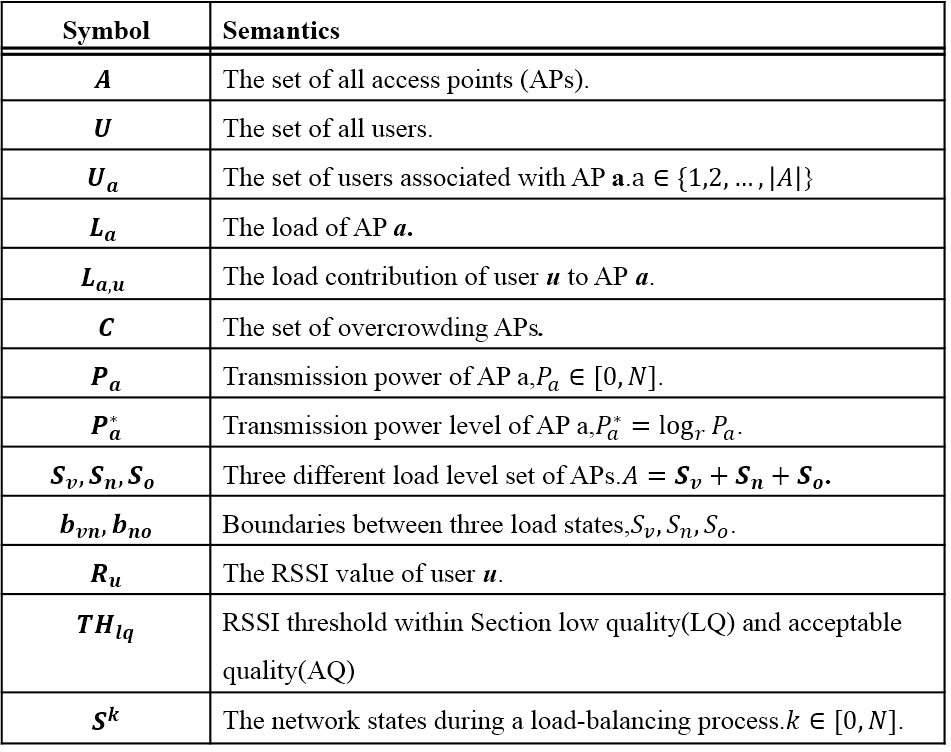
\includegraphics[width=3.4in]{images/notations.png}
% \end{table}

\begin{table}[tbp] 
    \normalsize
    \caption{Notations} 
    \begin{center} 
        \label{tab: Notations} 
        \begin{tabularx}{\linewidth}{| c | X | } 
            \hline \textbf{Symbol}  & \textbf{Semantics} \\ 
            \hline $A$              & the set of all access points (APs) \\ 
            \hline $U$              & the set of all users \\ 
            \hline $U_a$            & the set of users associated with AP $a$, $a \in$ \{1, 2, ..., $|A|$\} \\ 
            \hline $L_a$            & the load of AP $a$ \\ 
            \hline $L_{a,u}$        & the load contribution of user $u$ to AP $a$ \\ 
            \hline $C$              & the set of overcrowding APs \\ 
            \hline $P_a$            & transmission power of AP $a$\\ 
            \hline $P_{a, max}$     & the maximum transmission power of AP $a$\\
            \hline $P_{a, min}$     & the minimun transmission power of AP $a$\\
            \hline $P^{*}_{a}$      & the transmission power level of AP $a$\\
            \hline $N$              & the number of transmission power level\\
            \hline $P^{*}_{a(lv.n)}$   & the transmission power level of AP $a$ at level $n$, $n$ $\in$ $[$0, $N]$\\
            %%  ==== comment by little six 2016/10/21 ==== 
            %%  (equation 1 would explain this)
            %, $P^{*}_a$ = $log_\gamma P_a$ \\ 
            \hline $S_v, S_n, S_o$  & three different load level set of APs, $A$ = $S_v$ + $S_n$ + $S_o$ \\ 
            \hline $b_{vn}, b_{no}$ & boundaries between three load state \\ 
            \hline $R_u$            & the RSSI value of user $u$ \\
            %%  ==== comment by little six 2016/10/21 ==== 
            %%  (not used in following description)
            % \hline $TH_{lq}$        & RSSI threshold within Section low quality (LQ) and acceptable quality (AQ) \\ 
            \hline $S^k$            & the network states during a load-balancing process\\
            %%  ==== comment by little six 2016/10/21 ==== 
            %%  (different definition of N)
            %, k $\in [$0, $N]$ \\ 
            \hline 
        \end{tabularx} 
    \end{center} 
\end{table}

Figure \ref{fig:scheme1} shows our system architecture. 
The notations used in our scheme are shown in Table \ref{tab: Notations}. 
We consider an IEEE 802.11 WLAN with a set of APs, which is denoted by $A$, and $|A|$ indicates the number of APs. 
All APs are attached to a wired infrastructure and an OpenFlow controller. 

In our scheme, we focus on the transmission power of AP beacon messages since beacon messages are used for AP association.
% to the AP selection of users. 
We denote transmission power of AP $a$ as $P_a$.
According to the configuration and ability, each AP has its maximum and minimum transmission power, denoted as $P_{max}$ and $P_{min}$ respectively. 
Each AP also provides several transmission power levels from $0$ to $N$, denoted by $P_{a(lv.n)}^*$. 
We denote $P_{a(lv.0)}^*=P_{a, min}^*$ as the minimum power level of AP, and similarly we denote $P_{a(lv.N)}^*=P_{a, max}^*$ as the maximum power level.
For normal commercial AP products, the transmission power level configuration follow that
%We define 
\begin{eqnarray}
{P_a^*}=log _\gamma\left({P_a} \right)  \quad,\gamma=\sqrt[N]{\frac{P_{max}}{P_{min}}}
\end{eqnarray}
Then $P_{a(lv.n)}^*$ is a geometric series which can be expressed as
\begin{align}
&P_{a(lv.k)}^*={P_{a(lv.k-1)}^*}*\gamma\\										
&P_{a(lv.k)}^*={P_{a, min}^*}*{\gamma^k}, k\in[0, N].							
\end{align}
In our scheme we have some assumptions. First, we assume that the interference between adjacent cells can be ignored. Second, we assume that the AP deployment ensures complete overlaps between the ranges of all APs. In other words, if all APs are configured to the minimum transmission power $P_{min}$, every user in network coverage area can be still covered.

When a mobile device joins a WLAN, it listens every channel for all beacon messages from APs. Then, it associates with an AP which has the strongest RSSI, which is determined by the beacon transmission power and the distance between AP and user. In our system, we use all APs to collect the RSSIs from users  (Figure \ref{fig:scheme1}). Each AP reports the RSSIs to the controller by using OpenFlow protocol. Once in a while, each AP collects its load $L_a$  and the load contribution of its users $L_{a,u}$  to controller. Based on the information above, the controller knows the association relationships between users and APs. In the same way, the load of APs is also known by controller. In our system, the controller has a global view of the whole network.

We use $U$ to denote the set of all users in the network coverage area and $|U|$ is total number of users in U. Each user associates with at most one AP at any time, and we denote $U_a$ as the set of users associated with AP $a$. In normal cases, if a large amount of user association requests are sent to an AP in a short time, the AP become overloaded seriously. To stress the coordination ability of APs, we consider the group arrival cases. We assume that all users follow a group mobility model in our system. The users usually move together from one place to another in several groups.

Owing to the global vision of controller, we design an adaptive load balancing model using association allocation. Our model can coordinate the load of all APs and take the users' load contributions into consideration. For example, the busy users, who need whole allocated bandwidth to upload or download data frequently, are considered. The controller records the load contribution of user $u$ to AP $a$, $L_{a,u}$ by considering the load report from APs. Each AP can provide different bandwidths to its associated users in our case.

%% Figure 3.1

\begin{figure}[tbp]
\begin{center}
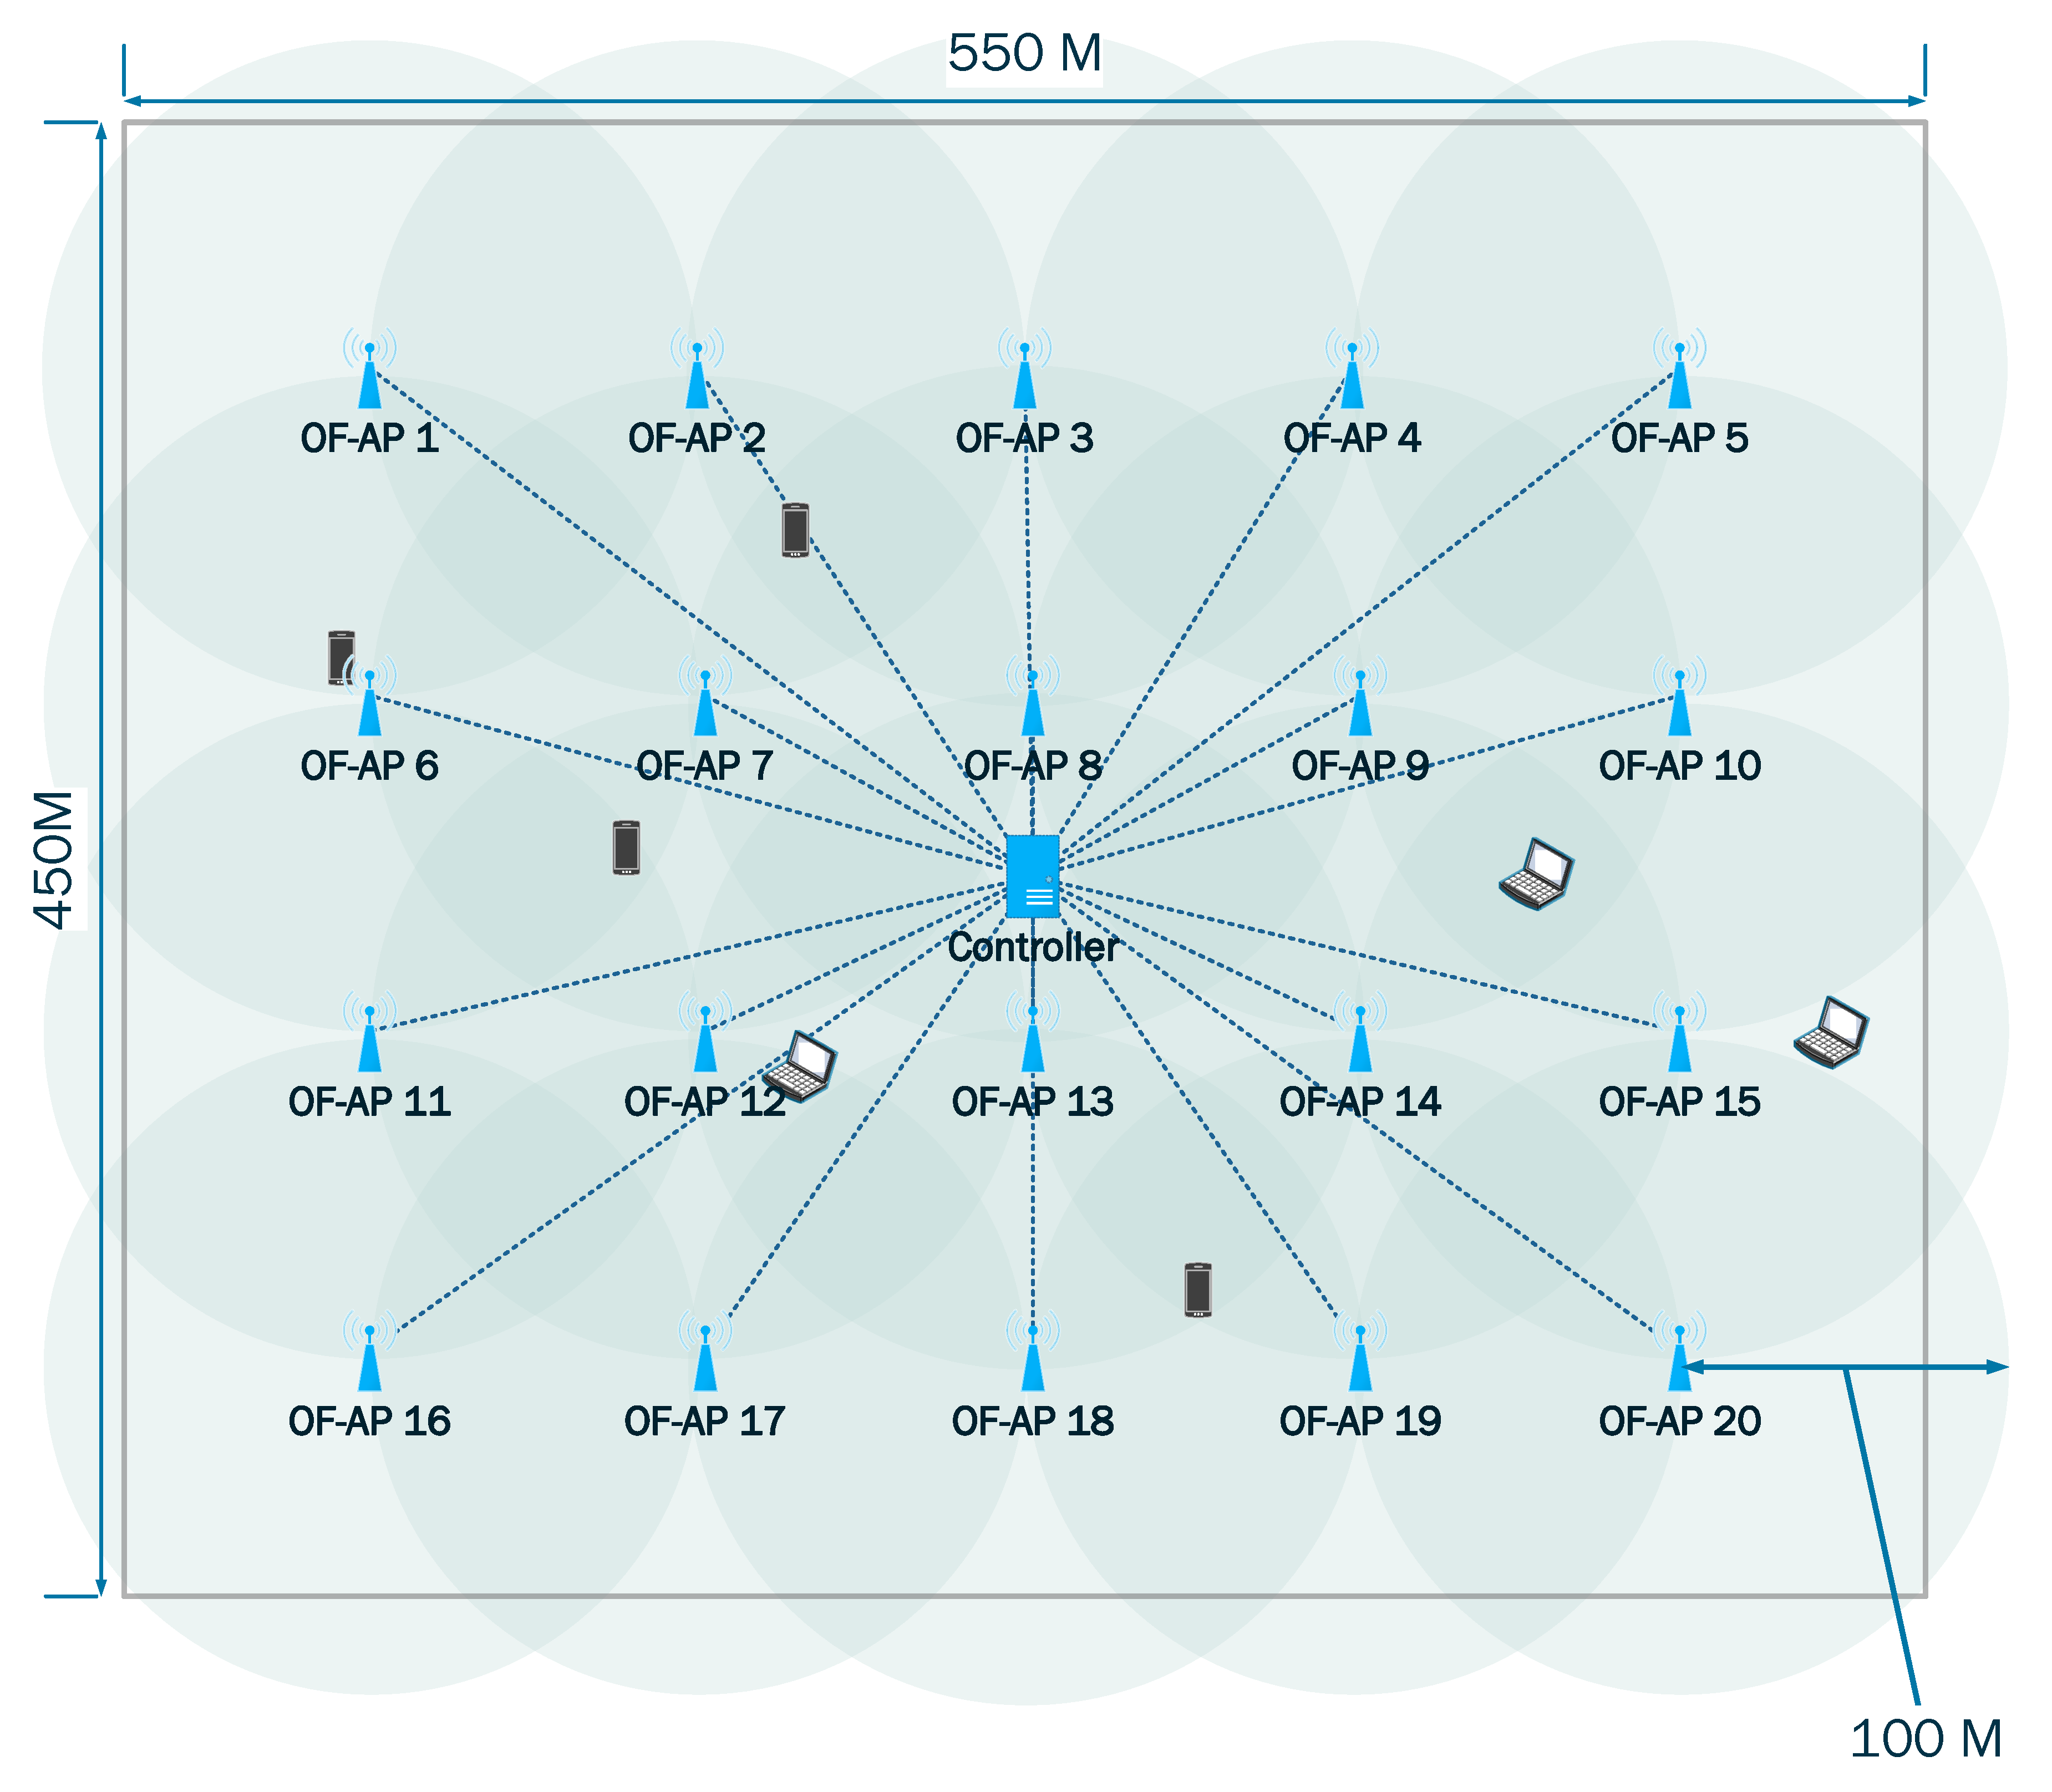
\includegraphics[width=3.4in]{images/scheme1.pdf}
\end{center}
\caption{System Architecture}
\label{fig:scheme1}
\end{figure}
%\clearpage

\subsection{Arrival Event Detection}\label{section:3.2}
In this subsection, we present the initial stage of adaptive load balancing. We design the procedures for APs to report its user association events and load in real time. Figure \ref{fig:flowdiagram_trendindicator_ap} shows the flow chart of AP reporting mechanism, and the steps are described below.

\begin{description}
  \item [Step 1.] Each AP records the user RSSI, user association list and its load periodically. All APs receive RSSIs in every authentication frames from their users.
  \item [Step 2.] If there is a new user associating with the AP, go to \textbf{Step 3}. Otherwise, go to \textbf{Step 4}.
  \item [Step 3.] The AP sends the user RSSI to the controller. Then go to \textbf{Step 6}.
  \item [Step 4 and 5.] If there is no new arrival in \textbf{Step 2}, the AP reports its load to controller periodically.
  \item [Step 6.] After sending report messages to controller, the AP would receive a Beacon-Config message from the controller.
  \item [Step 7.] The AP configures its beacon transmission power.
\end{description}

%% Figure 3.2
\begin{figure}[tbp]
\centering
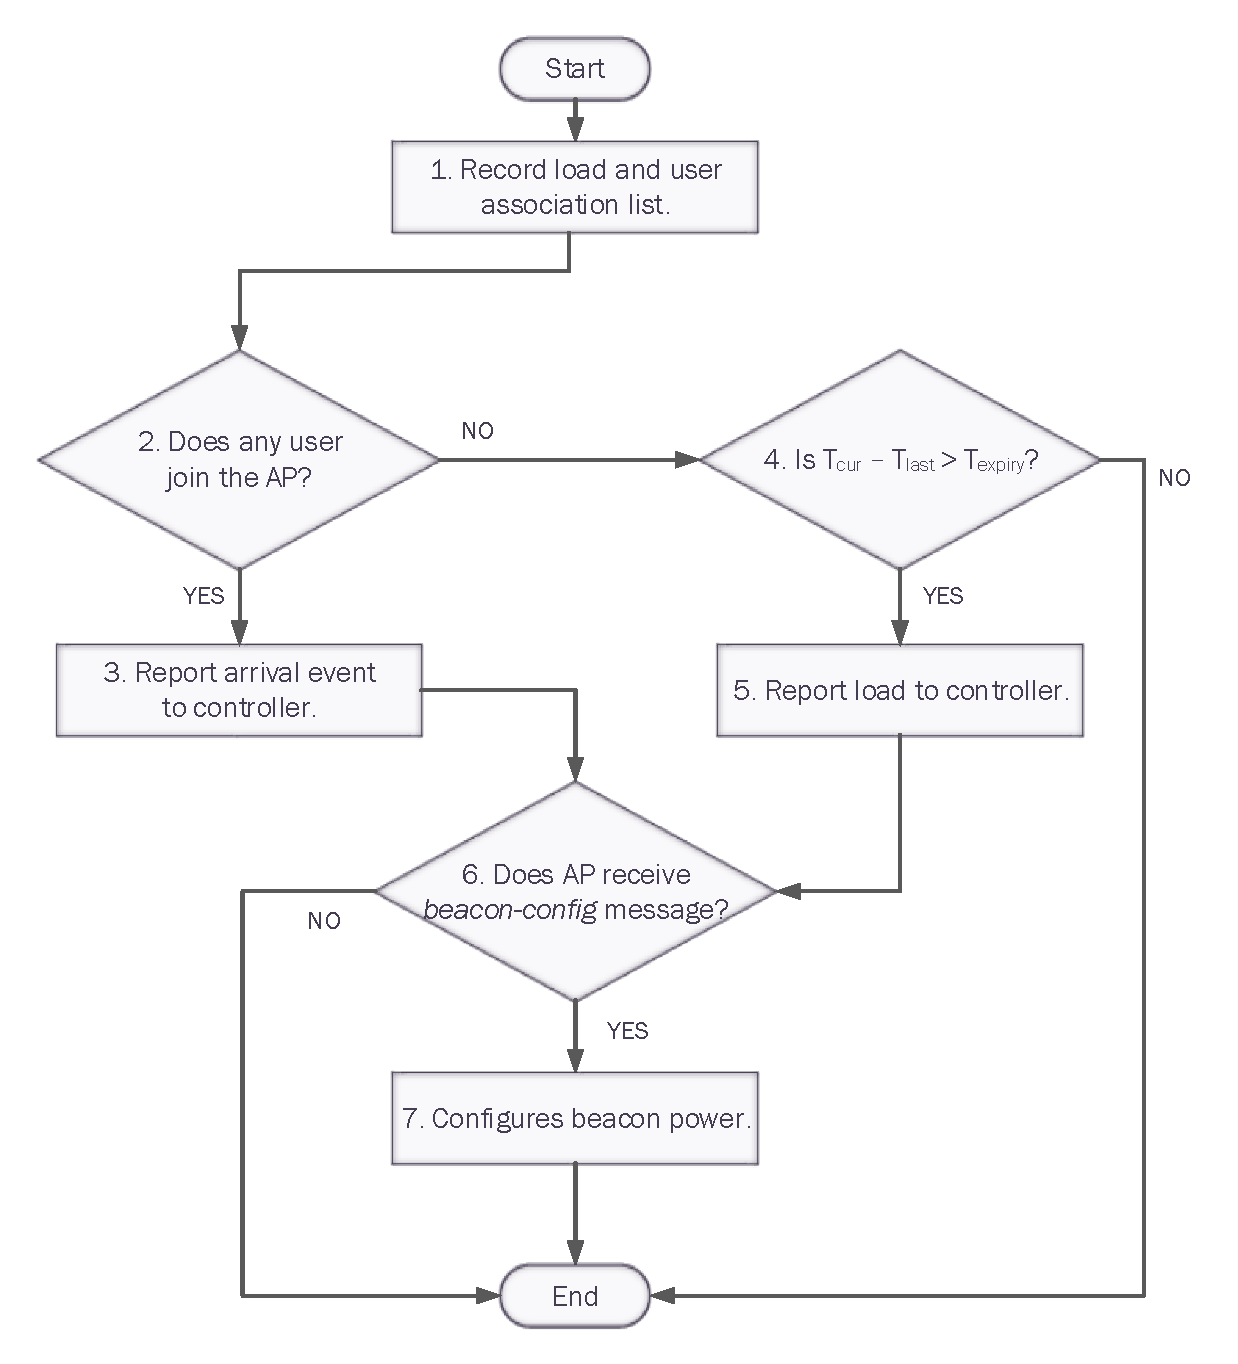
\includegraphics[width=3.4in]{images/flowdiagram_trendindicator_ap.pdf}
\caption{Flow Chart for AP Reporting Mechanism}
\label{fig:flowdiagram_trendindicator_ap}
\end{figure}

%\clearpage
% comment out by little six 2016/10/14
%On the other side, we describe a flow chart of controller manage mechanism in Figure \ref{fig:flowdiagram_trendindicator_controller}.
The flow chart of the controller management mechanism is shown in Figure \ref{fig:flowdiagram_trendindicator_controller}, and following is the descriptions of steps.

\begin{description}
  \item [Step 1.] The controller receives arrival events and load messages from APs.
  \item [Step 2.] The number of new arrival events is added into the arrival counting table. Then the controller calculates event increase at the latest time interval.
  \item [Step 3.] The controller compares the number of current arrival events with the past. When an AP exceeds the threshold of arrival events, it has a high risk of overcrowding. At this time, the controller gives the AP a predicted load value and then go to \textbf{Step 6}.
  \item [Step 4.] The controller classifies all APs into three load levels: vacant, normal and overcrowding. According to the levels, the APs are added into $({S_v}$, ${S_n}$ and ${S_o}$) respectively. The $b_{vn}$ and $b_{no}$ denote the boundaries between these levels.

      \begin{align}
        &L_{l,a}=\left\{\begin{array}{lll}
            v, L_a \leq b_{vn} \\ n, L_a \leq b_{no} \\ o, L_a < b_o
            \end{array} \right\} \\
            \nonumber\\
        &S_v={a|L_{l,a}=v}\\
        &S_n={a|L_{l,a}=n}\\
        &S_o={a|L_{l,a}=o}
      \end{align}
  \item [Step 5.] This procedure ends when there is no AP changing to overcrowding state $S_o$.
  \item [Step 6.] The controller calculates the adjustments of APs according to the load balancing algorithm which is described in next subsection.
  \item [Step 7.] The controller send a beacon-config messages to each AP.
\end{description}

%% Figure 3.3
\begin{figure}[tbp]
\begin{center}
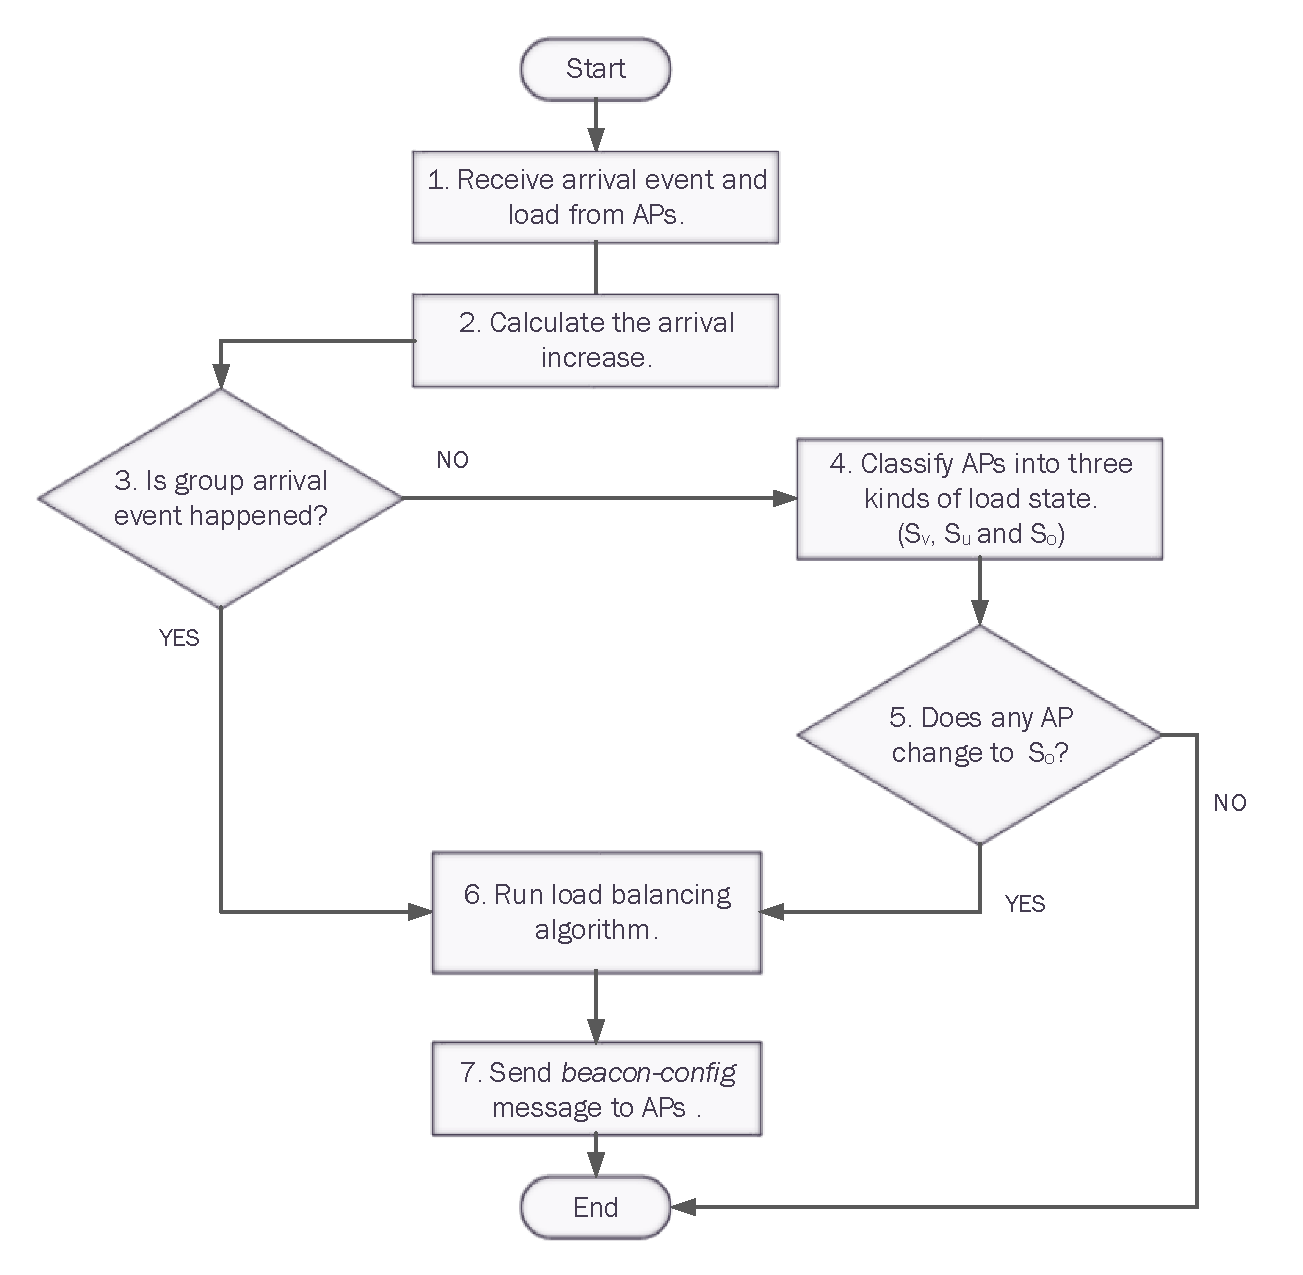
\includegraphics[width=3.4in]{images/flowdiagram_trendindicator_controller.pdf}
\end{center}
\caption{ Flow Chart for Controller Management Mechanism}
\label{fig:flowdiagram_trendindicator_controller}
\end{figure}
%\clearpage

\subsection{Adaptive Load Balancing}
In this subsection, we present the adaptive load balancing mechanism. Recall what we described in subsection \ref{section:3.1} and \ref{section:3.2}, the association relationship, RSSIs of users and load of APs are all collected by the controller. Based on the information above, the controller has a global vision of whole wireless network. We combine SDN and Cell-Breathing method into an Adaptive Load Balancing mechanism.

 Figure \ref{fig:algorithm} shows the pseudo code of our mechanism for controller. In this algorithm, the beacon power level is first initialized to the maximal power level. The controller collects and calculates the summations of all AP utilizations, and the network state is initialized as $S^0$. First, the algorithm iteratively finds the most overcrowding AP. Then, the most overcrowding AP is added into overcrowding set $C$ and sets its power one level down. In the meanwhile, the adjustment is recorded in a stack structure. Every time the most overcrowding AP sets down beacon power level, the algorithm updates the AP states by simulating the association relationship between APs and users. Each state is compared with previous states to find the optimal state. Until the iteration ends, the algorithm sets all AP beacon power level according to the optimal state.

This algorithm terminates in two conditions. The first condition is that the overcrowding set $C$ is equal to AP set $A$. When these two sets are equal, every AP is adjusted. At this time, the results are the same, even though the iteration continues. The second condition happens when any AP beacon power level is zero. If the iteration continues, some APs can not trun down their beacon power anymore, thus they become overcrowding again.

%% Algorithm
\begin{figure}[tbp]
\centering
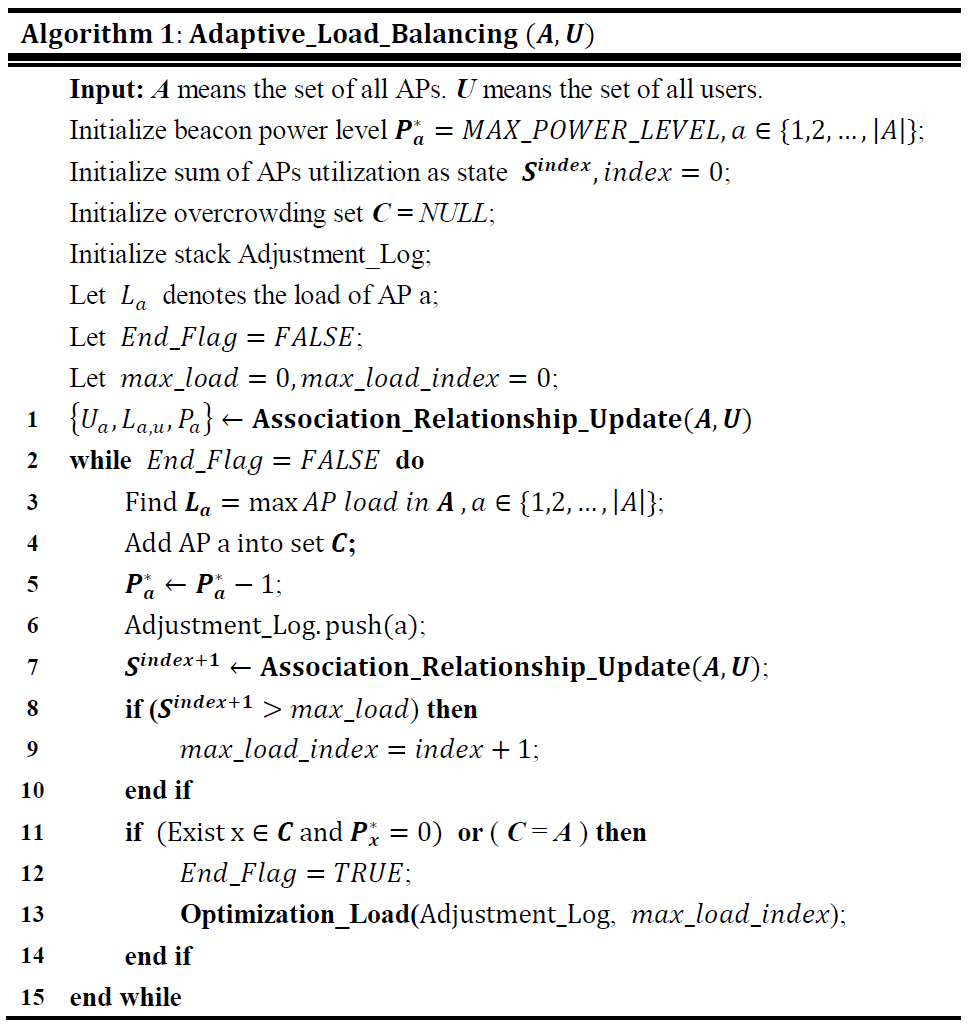
\includegraphics[width=3.4in]{images/algorithm.png}
\caption{Adaptive Load-Balancing Algorithm}
\label{fig:algorithm}
\end{figure}
%\clearpage

Figure \ref{fig:flowchart_Cell_Breathing} illustrates the message flow of association control between users, APs and controller. We assume that user is in the coverage of AP 1 and 2, and AP 1 is closer to user than AP 2. We assume that the user has passwords of AP 1 and AP 2. Both these two APs connect to controller via secure channel.

\begin{description}
  \item [Step 1.] AP 1 and AP 2 send Beacon Message to the user periodly.
  \item [Step 2.] AP 1 and AP 2 report their load (utilization) and association events to controller. In OpenFlow protocol, association event can be transmit in Packet\_In message and the load of AP can be transmitted in Port\_Status message.
  \item [Step 3.] Controller periodly checks all of the AP load and integrates all association event reports of APs. Then controller inputs these information to Adaptive Load Balancing program.
  \item [Step 4.] Based on the result of \textbf{Step 3}, controller sends Beacon-Config messages (i.e. SetConfig message in OpenFlow) to APs. In this case, controller decides to reduce load of AP 1, thus controller sets the AP 1 beacon power lower than AP 2 beacon power.
  \item [Step 5.] The same as \textbf{Step 1}, AP 1 and AP 2 send beacon message to the user.
  \item [Step 7-9.] The user sends association request to AP 2, which has the highest RSSI. After receiving an association response from AP 2, user sends an authentication request to AP 2. When AP 2 sends back authentication response, the connection between user and AP 2 is established.
\end{description}

%% Figure 3.4
\begin{figure}[tbp]
\begin{center}
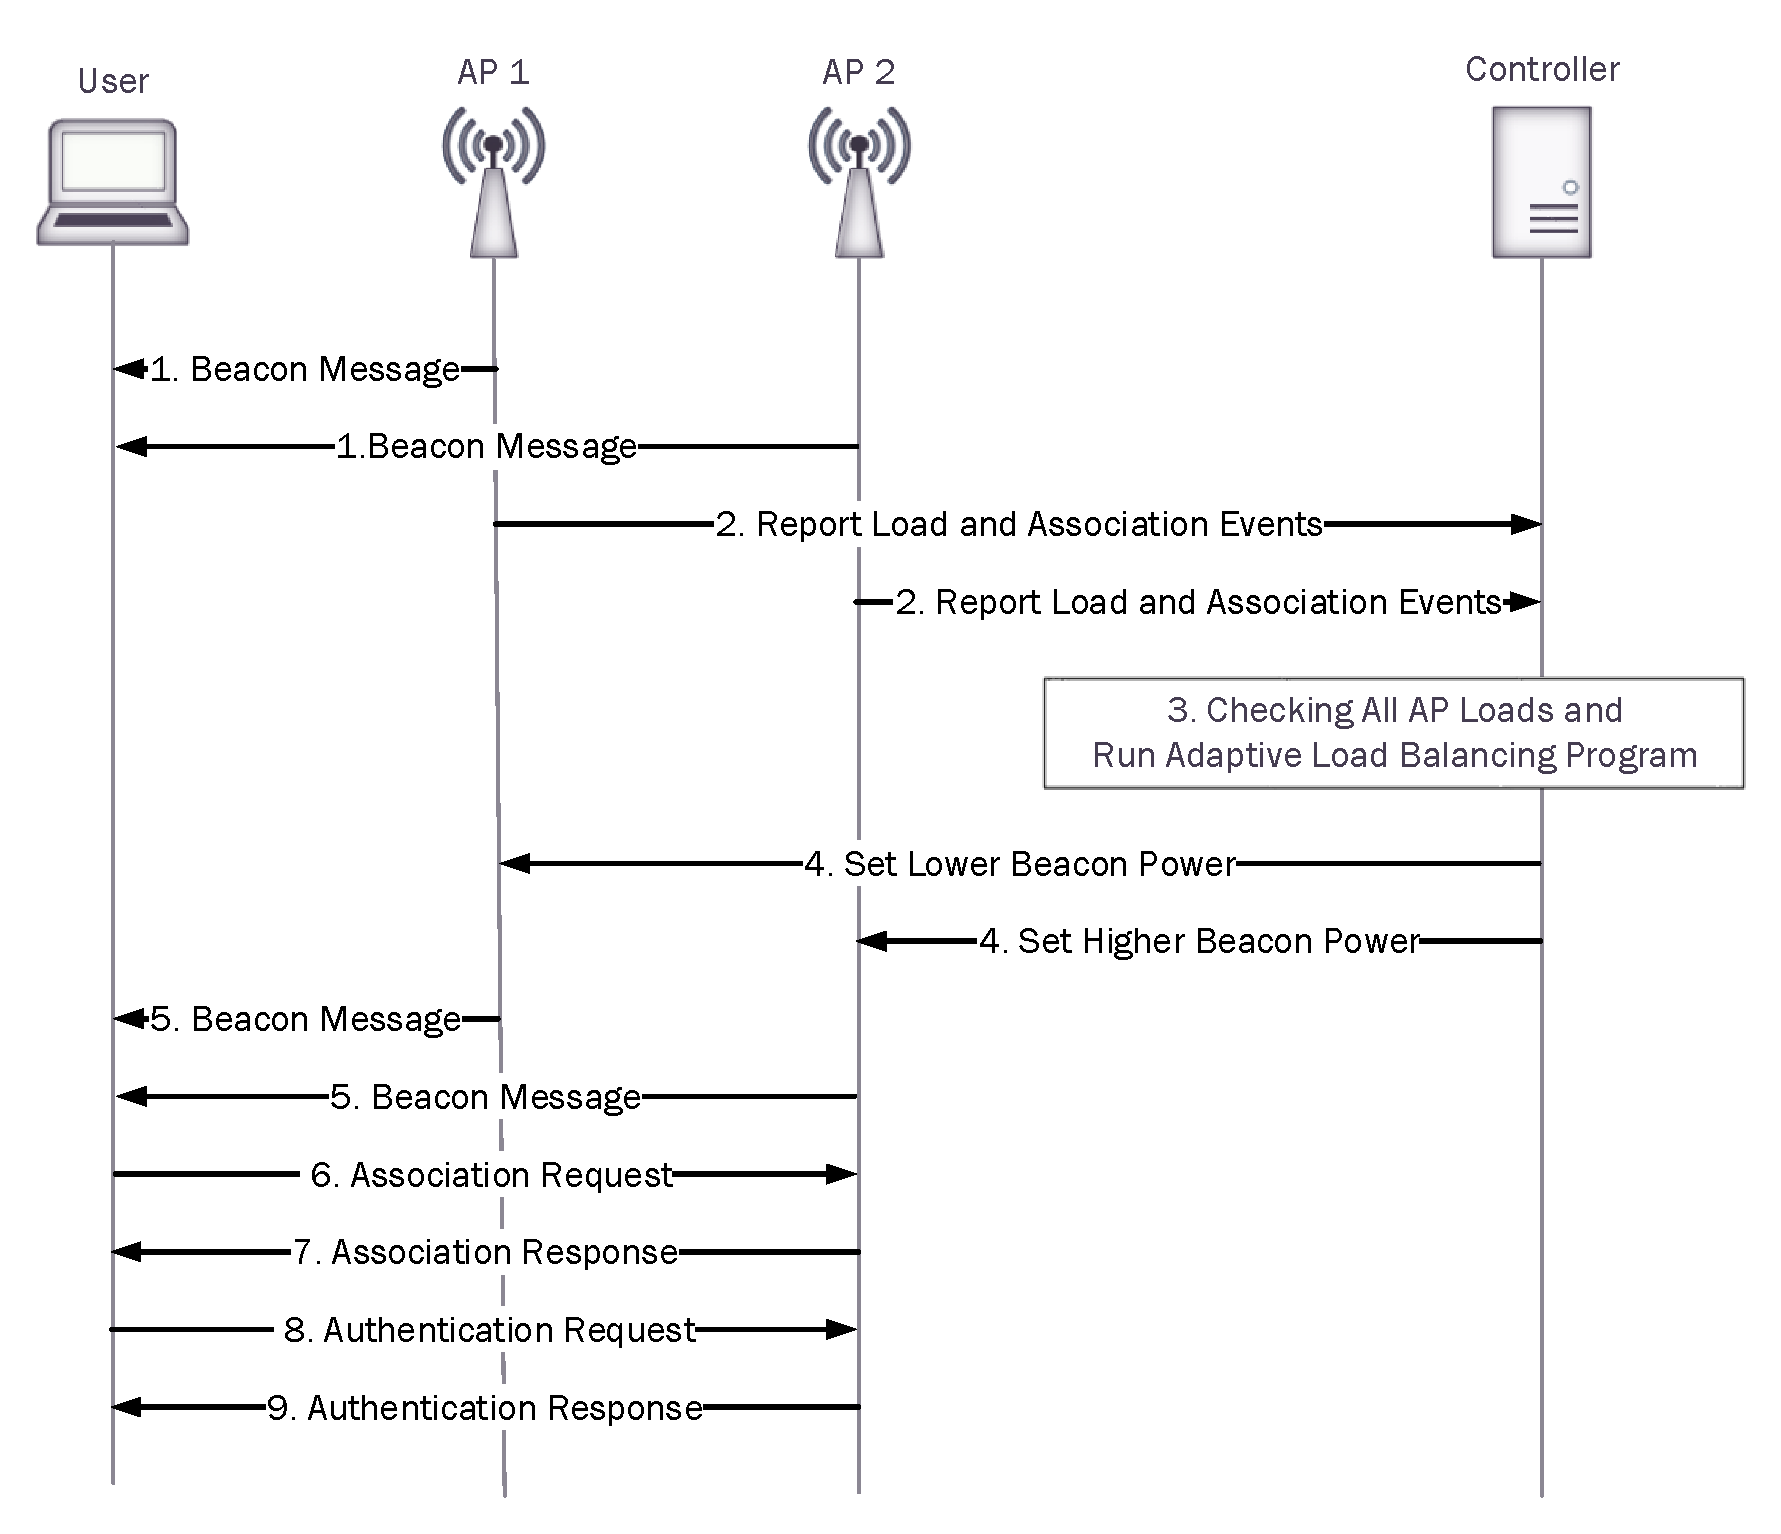
\includegraphics[width=3.4in]{images/flowchart_Cell_Breathing.pdf}
\end{center}
\caption{Message Flow of Association Control}
\label{fig:flowchart_Cell_Breathing}
\end{figure}

% above Dotto


